\documentclass{article}
\usepackage[utf8]{inputenc}
\usepackage[dvipsnames]{xcolor}
\usepackage{hyperref}
\usepackage{verbatim}
\usepackage{graphicx}
\usepackage{fancyhdr}

\pagestyle{fancy}
\fancyhf{}
\lhead{Digital Methods by Victor Harbo Olesen}
\rhead{Studienr: 201705028}
\rfoot{Page \thepage}

\title{Proof of Concept}
\author{Victor Harbo Olesen}
\date{08/01/2020}

\begin{document}
\maketitle

\section{Abstract}
This proof of concept will show how it is possible to extract highlights, annotations, highlights with annotations, notes and other edits from PDF-files. The script used for this is a python script, but it is possible to run it in an R environment. This extracting of data can be helpful when taking notes as a student or even when writing assignments and articles on a higher level. The script has the ability to extract highlights, annotations, highlights with annotations and also underlined annotations. It is a versatile tool that can be used for taking notes, producing quotes for papers and it can also be used for reviewing.
\section{Keywords}
Python; PDF; pdfannots; pdfminer.six; R; RStudio; Reticulate; Python and R; textmining; tm; 
\section{Introduction}
Have you ever read an article in the form of a .pdf file and wanted to extract your notes afterwards?
This script does exactly that with a few commands. This script is not only relevant for historians, but for everyone who from time to time reads and annotates PDF’s, this could be anyone from professors at a University to High School students. Andrew Baumann, the author of the original python script, which this script is based on, has made the code to make his reviewing of conference papers easier. As said before I believe it is a great annotation tool for notetaking as well. \newline
To make use of this script, you would have to download the correct version of Python for your computer and be able to install a python package called pdfminer.six. That is as little python needed for making this script run. The rest will happen in R. In terms of skills it would be an advantage to know how to navigate your filesystem through bash. This is important because it will enable you to tell the script where the PDF file the you want to extract is located. \newline
The script and its dependencies are all available at my Github repository pdfannots\textunderscore in\textunderscore R at \url{https://github.com/Digital-Methods-HASS/au590745_Olesen_VictorHarbo}. My script is an R version of Andrew Baumanns pythonscript which is also available in my Github, but to get the original pythonscript for running it in python go to \url{https://github.com/0xabu/pdfannots}. When reading through this proof of concept I recommend having the script pdfannots\textunderscore inR.R open in RStudio and following along there as well. The script should be useable without this text, but some parts of this paper might not make much sense without the script to look at as well. 

\section{Problems and background}

The script used in this proof of concept has no historical background and is not directed at a specific historical period or event. Instead it is a tool developed for researchers and students in general. As mentioned in the introduction this tool can solve a notetaking problem, which for me until this course had been frustrating. It allows you to extract annotations and highlights from PDF-files.
As a result of the paper not being directed at any historiography but rather being a universal tool, the literature for this assignment is not dominated by articles, books etc. regarding history. In fact most of the references in this paper are going to be referring to web pages and video-tutorials that have helped me understand Python and scripts in general.
The most important reference for this paper is Andrew Baumann and his GitHub repository at \url{https://github.com/0xabu/pdfannots}. Baumann is the author behind "pdfannots" which is the script that allows the end-user to extract highlights and annotations from PDF's. Besides Baumann, Emma Rand and her repository on running python in R has been of great use for this project. This can be found at \url{https://github.com/3mmaRand/useR2019_tutorial}

\section{Software framework}
\subsection{Choice of software}
It does not matter if the script is run directly in python through bash or through the R package reticulate. The choice depends on what software the user is using already and if installing python for bash would clash with other versions of python that might be installed. Personally I am using the script in R, because R is what we have been taught in our class. I have run this script on a PC running a 64-bit version of windows 10. To be able to run the python script trough R I have used R version 3.6.1, RStudio version 1.2.5019 and Python Anaconda 3.7.4. When I tried running the script directly in python through bash I used Python 3.7.5, installed from pythons own windows 64-bit installer, found at \url{https://www.python.org/downloads/windows/}.

\section{Data Acquisition and Processing}
As this paper is not doing data driven history but rather assessing a practical obstacle for everyone doing digital textual work. This tool does require some data to run on, which is the PDF-file with annotations. This can be anything and in my own case I will use a PDF on medieval heresy and inquisition because it is relevant for another paper I am currently working on. If anybody wants that specific document it is "A History of Medieval Heresy and Inquisition" by Jennifer Kolpacoff Deane. The part of it that I am using as the example is the introduction. I have annotated this PDF with my own notes, which can be seen as the processing of the file. Again, this PDF could be any PDF that is useful for you.

\section{Implementation and Empirical Results}
In this section it will be shown how to get Python running in R. To do this I followed Emma Rands tutorial on "Keeping an exotic pet in your home" which can be found at \url{https://github.com/3mmaRand/useR2019_tutorial}. From here the paper will move towards using the actual script and avoiding the common pitfalls that seems to exist.  
\subsection{Getting started with Python}
The pdfannots script is written in python, which makes python a requirement for using the script to extract data from PDF’s. When the script is run through R, python is still needed on your computer. Very little action is made in python. For downloading anaconda to be used in R follow this guide closely \url{https://docs.anaconda.com/anaconda/install/}, when anaconda has been successfully installed open up the anaconda prompt on your system and type: 
\begin{verbatim}
    pip install pdfminer.six
\end{verbatim}
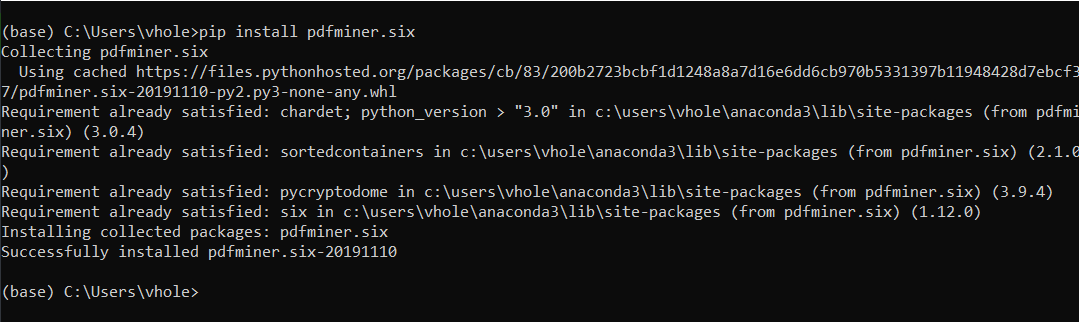
\includegraphics[scale=0.53]{Install_pdfminer_six.PNG}\newline
It has been done successfully when the last thing the prompt says is: "successfully installed pdfminer.six". From here everything you have to do is happening in R. Python is all set up for doing what it does in the background. Now the paper will work towards using python through RStudio

\subsection{R and RStudio}
R is the program that we have been using during this course and therefore it seems natural to make this script available to be used through R. Making the script usable through R hopefully allows people who are more comfortable in R to use the script as well. To run python in R the package "reticulate" is required. This can be downloaded by running this line in RStudio:
\begin{verbatim}
    install.packages("reticulate")
\end{verbatim}
If this warning is shown, try installing the package Rtools as well: \textit{WARNING: Rtools is required to build R packages but is not currently installed. Please download and install the appropriate version of Rtools before proceeding:} Rtools can be installed like this:
\begin{verbatim}
    install.packages("Rtools")
\end{verbatim}
When reticulate is successfully installed python can be run in R. In my Github repository there is an R-script containing the pieces of code that makes the pdfannots script run in R. The normal console in RStudio is showing a single \textgreater, when running python in R it changes into \textgreater\textgreater\textgreater. To run basic python commands in R we have to use the command:
\begin{verbatim}
    repl_python()
\end{verbatim}
When this is done. The console in R should look like this: \newline
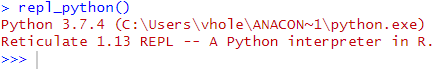
\includegraphics[scale=1]{repl_python.PNG} \newline
Here R tells us, that it ran the command and it has detected python version 3.7.4 in the specified path. When \textgreater\textgreater\textgreater is shown, it means that the console takes python inputs. To return to the console that understands R inputs, simply type in:
\begin{verbatim}
    quit
\end{verbatim}
You have now exited the reticulate python console and are back in the normal R console. This opening and closing of reticulate python is useful to understand how to navigate between Python and R. This command is actually \textbf{not} required when running the pdfannots.py script.This is because the script needs to be run with another command, more on this later.\newline
This was a short description on how to run python in R. If anything is causing trouble, consult the slides of Emma Rand at \url{https://3mmarand.github.io/useR2019_tutorial/#38} \newline
A very important part of getting Python and R to work together is setting an environment variable in windows. This is done by doing as Emma Rand points out in her tutorial located at \url{https://github.com/3mmaRand/useR2019_tutorial}
\begin{itemize}
    \item You need to set your QT\textunderscore PLUGIN\textunderscore PATH environment variable to where the RStudio and Anaconda3 plugins are located
    \item In windows: Control Panel -\textgreater System and Security -\textgreater System then
    \item Advanced System settings -\textgreater Environment variables
    \item I have set mine to:
    \item \begin{verbatim}
C:\Program Files\RStudio\bin\plugins; C:\ProgramData\
Anaconda3\Library\plugins  
    \end{verbatim}
    \item \begin{verbatim}You may need to add a new variable. The order of the paths
matters - make sure you have the C:\Program Files\RStudio
\bin\plugins first.
    \end{verbatim}
\end{itemize}

\subsection{Pdfannots.py in R}
This section of the text will focus on how to install the script, where to put it in your system, how to use it through RStudio and things to remember when working with the script. First things first. We have to have access to the script in order to use it. The script was originally made by Andrew Baumann and it can be found in his GitHub repository at \url{https://github.com/0xabu/pdfannots}. I have also uploaded the script to my GitHub repository, which can be found here: \url{https://github.com/Digital-Methods-HASS/au590745_Olesen_VictorHarbo/tree/master/pdfannots_in_R/input}, so that it is easy to find both this paper and the script it is about at the same place. All credit for the pdfannots.py script goes to Andrew Baumann. 

\subsubsection{Accessing the script}
At first I found the script on GitHub through a search on the words "pdf" and "annotations". From here I cloned the repository to my computer through bash with the command:
\begin{verbatim}
    git clone \url{https://github.com/0xabu/pdfannots}
\end{verbatim}
Now I had the repository with the link cloned to my computer. In R you have the ability to open python scripts, so I did that and had a look at the script. It looks like this in the beginning: \newline
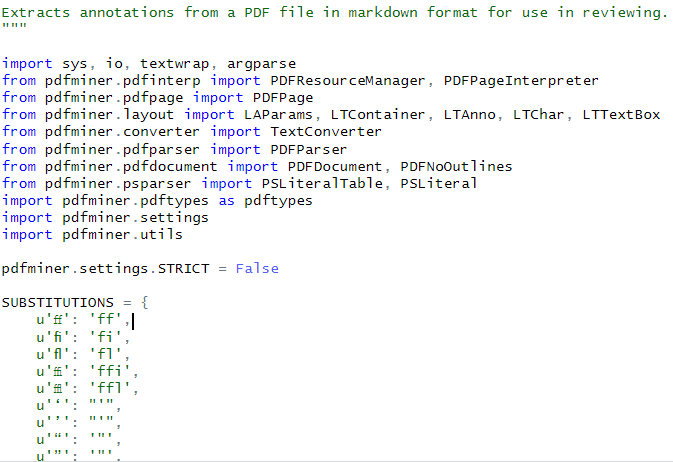
\includegraphics[scale=0.85]{part_of_pdfannotspy.PNG} \newline
I tried to figure out if there was anywhere I had to put a path to the file I wanted to run the script on, but could not figure out where that should be, so I started searching for some of the different parts of the script. It turns out that the part of the script regarding argparse is a way to tell python that it needs an argument input. This means that the script is built in a way so that you do not have to change anything in it when changing files. The only thing you have to change when changing files is the path to the input file, written in the console command. More on that later. At first you have to be sure that the script is in the right place. The script has to be placed in the same working directory as where we are running the R-package reticulate. I like to import the PDF's into a folder in the same working directory called input, just to keep everything in order and in the same place. \newline
With R being able to understand a python script, the pdfannots.py script in the right directory and with an annotated PDF we are finally ready to run the script.

\subsubsection{Running the script}
As mentioned earlier, there are many ways to communicate with python through the reticulate package. To make the script run we have to use the command:
\begin{verbatim}
    system("python pdfannots.py PATH TO FILE")
\end{verbatim}
To make the script run from this we have to specify where the file is located. I have my PDFs in the input folder of my working directory. In this folder I have a file named "a\textunderscore history\textunderscore of \textunderscore medieval\textunderscore heresy\textunderscore and\textunderscore inquisition.pdf" because I am doing another paper on medieval heresy at the moment. In this text I have made a lot of highlights and annotations  and I would like to have them in plain text. So to run the script on this file I would write this piece of code:
\begin{verbatim}
    system("python pdfannots.py input/a_history_of_medieval_
    heresy_and_inquisition.pdf")
\end{verbatim}
Running that line gives a result looking like this:\newline
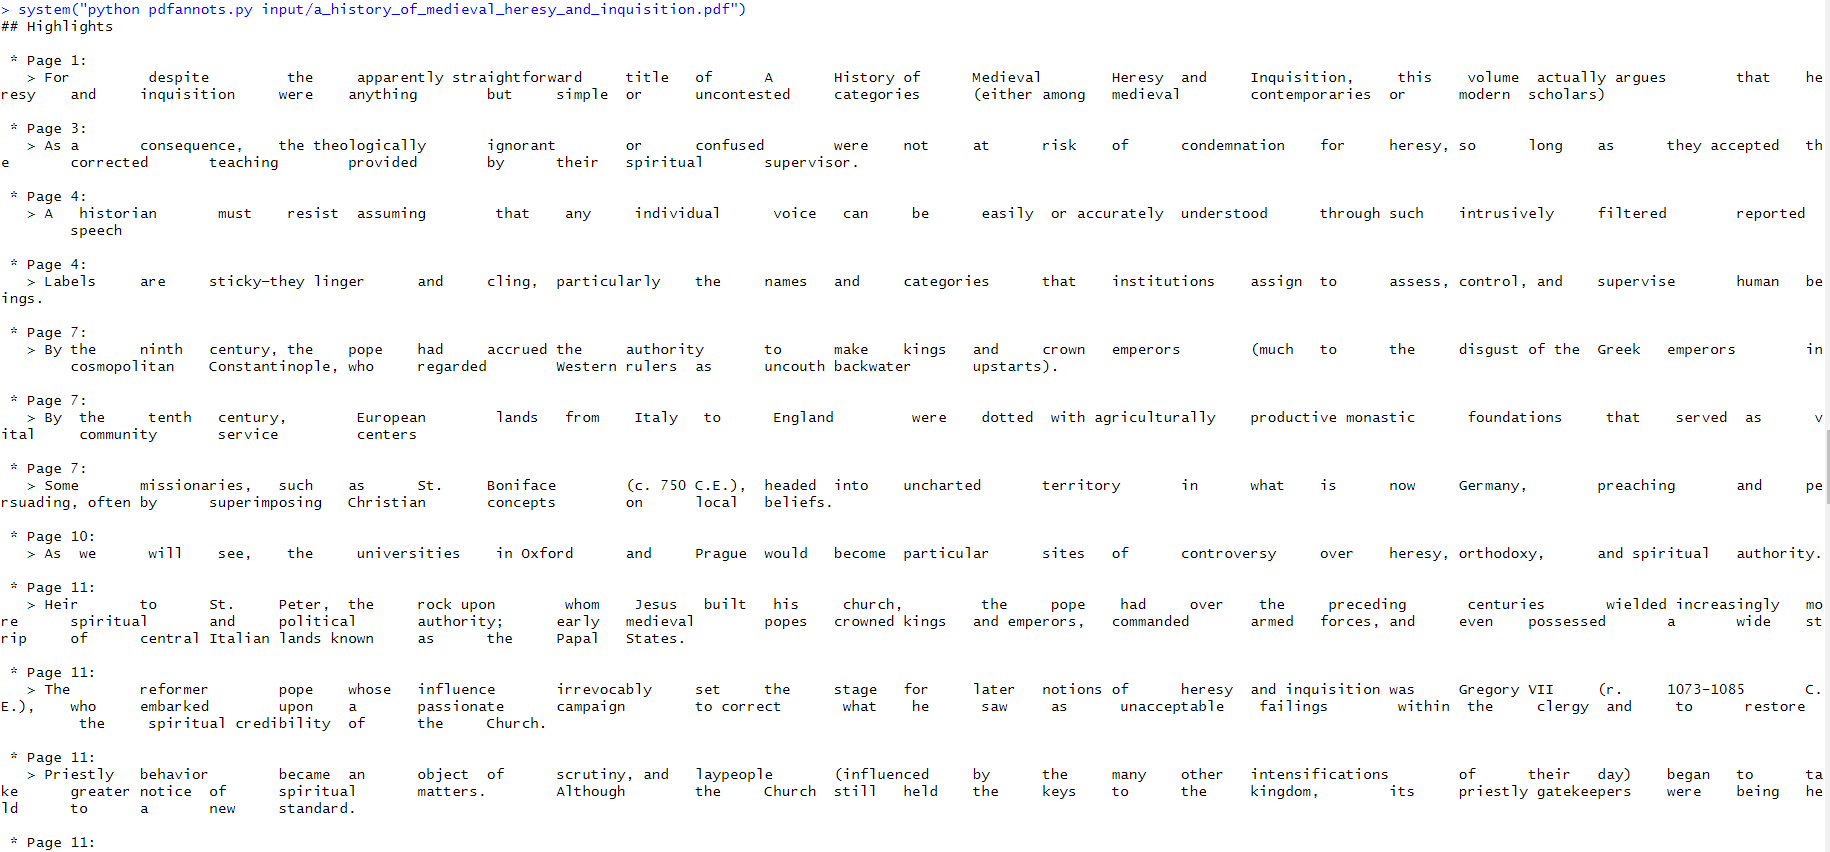
\includegraphics[scale=0.5]{result_of_running_code.PNG} \newline
The output is all of my highlights, annotations and underlines in that PDF-file. The console does detect a lot of spaces in the PDF and the annotations. For these I have a little work around using regular expressions. Another way to run the script, which is actually more efficient, because it makes an output file is to run the command like this:
\begin{verbatim}
    system("python pdfannots.py -p -o output.txt input/ 
\end{verbatim} \newline
\begin{verbatim}
    a_history_of_medieval_heresy_and_inquisition.pdf")
\end{verbatim}
It runs the script, but it gives the output in the file output.txt. This is possible because of the -o flag and then the name of the new file afterwards. The -p flag shows the progress of the script in the console. This enables us to see what the script detects when it is run on the PDF.

\subsubsection{Making the output readable}
As mentioned above, the output of the script might be filled with lots of spaces and tabs. These can be removed by using regular expressions. This is done in the part of the script called textcleaning. When the script is run on other files and has to be cleaned in any way it is easy to add or change those regular expressions used. Simply add another line in the code or change the things to substitute it. Right now the script removes \textbackslash t and replaces those with a single space, while it also substitutes multiple spaces with a single space. If you wanted to add another regular expression to the cleaning it could be done adding another of these lines:
\begin{verbatim}
for (j in seq(docs)) {
    docs[[j]] <- gsub("\t"," ", docs[[j]]) 
    docs[[j]] <- gsub(" +"," ", docs[[j]])
}
\end{verbatim}
An example could be to also remove all single digits, which could be done this way:
\begin{verbatim}
for (j in seq(docs)) {
    docs[[j]] <- gsub("\t"," ", docs[[j]]) 
    docs[[j]] <- gsub(" +"," ", docs[[j]])
    docs[[j]] <- gsub("\d","", docs[[j]])
} 
\end{verbatim}
These regular expressions are a part of the R package "tm" which is a textmining package, that is used in my script. Installation of tm and the steps prior to these regular expressions are all annotated in my script. 

\section{Critical evaluation}
This part of the paper will consist of some critical observations on the abilities of the script. There is one main concern regarding the pdfannots.py script. This is the scripts ability to recognise text in different PDF files. When feeding the script a PDF-file that is not born-digital the script might have a hard time figuring out what words, the highlights are actually highlighting, resulting in some weird extracted highlights. When that is said, general comments and annotations made in these "lower quality" PDF-files are exported flawlessly. The script definitely works best on born-digital material. My experience with it shows that it works on digitised material that is scanned in high quality and has an OCR layer.\newline
I do not know of any programs that allows me to extract annotations from PDF's like this script does. It is a feature I have looked for a couple of times and I am really grateful for finding this script and now being able to use it.

\subsection{The learning process}
The process of finding and learning to use this script has been a great experience. Before I started this course I had minimal experience with using my computer as a professional. The wildest thing I had used the computer for was making simple excel files and longer essays in word. Now I have learned programs as R, OpenRefine and proper usage of bash through the course. Furthermore during the process of getting this script to work I have learned how to run python scripts and even how to run these scripts in R. I find it useful that I have come to be able to use a script like this, which I am sure that I will make use of for the rest of my time at university.

\section{Conclusion}
It is possible to extract highlights, annotations and more from PDF-files. This can be done with the python script pdfannots. This script can be run through R with the R-package "reticulate". For people who are doing different things in R and python, being able to run the script in both places gives a huge bonus. The script is useful for a variety of different people. It is not only usable for historians. This script can be used by everyone who has use for annotating PDF-files. It does not matter if the PDF contains an article on micro history or microbiology. The script can be used for both notetaking, quotation findings and paper reviewing. It is a versatile tool, once you learn how to use it. The PDF-files given to the script do need to be of some quality to guarantee a meaningful result. Furthermore the script does produce a lot of blanks in the result, these are not an actual problem because they can be removed quickly by the use of regular expressions. 

\section{Acknowledgements}
At last I would like to thank Adela Sobotkova for her almost endless amount of consultations, which have helped me alot to understanding how to combine different parts of different scripts to end at this final result. Without these consultations I would never have been able to  produce an output file of any form. 
\newpage


\section{References}
Baumann, Andrew; pdfannots; at: \url{https://github.com/0xabu/pdfannots} \newline
Badger0053; Answer; at: \url{https://stackoverflow.com/questions/41638558/how-to-call-python-script-from-r-with-arguments}\newline
Rand, Emma; useR2019\textunderscore tutorial at: \url{https://github.com/3mmaRand/useR2019_tutorial} \newline
Sobotkova, Adela; TextMiningTutorial at:\newline
\url{https://github.com/adivea/TextMiningTutorial} \newline
Feinerer, Ingo; Rforge for tm package at \url{https://rdrr.io/rforge/tm/} \newline
\end{document}